
\section{Introduction}
\label{sec:introduction}
%%% General intro
\IEEEPARstart{T}{here} is a growing demand for ubiquitous AI sensor data analytics. Industry 4.0 and smart city infrastructure leverage AI solutions to increase productivity and adaptability\cite{lom2016industry}. These solutions are powered by advances in machine learning (ML), hardware engines, and big data. Hence, enhancement of these should be considered for research, as they are the machinery of the future.

CNN-based models represent the essential building blocks in 2D pattern recognition tasks. Sensor-based applications such as mechanical fault diagnosis\cite{li2019sensor,dong2018rolling}, structural health monitoring (SHM)\cite{nagayama2007structural}, human activity recognition (HAR) \cite{wang2019deep}, hazardous gas detection\cite{kim2017hazardous} have been powered by CNN models in industry and academia.

CNN-based models, as one of the main types of artificial neural networks (ANNs),
have been widely used in sensor analytics with automatic learning from sensor data \cite{ince2016real, janssens2016convolutional, abdeljaber2017real, guo2016hierarchical}. In this context, CNN models are applied for automatic feature learning, usually, from 1D time series as well as for 2D time-frequency spectrograms. CNN models provide advantages such as local dependency, scale invariance, and noise resilience in data analytics. However, these models represent compute-intensive and power-hungry tasks, particularly, for low-power and resource-limited Internet-of-Things (IoT) devices.

Dedicated hardware architectures are typically used to enhance compute performance and power efficiency. In terms of computational throughput, graphics processing units (GPUs) offer the highest performance. In terms of power efficiency, ASIC and FPGA solutions are well known to be more energy efficient (than GPUs) \cite{nurvitadhi2017can}. As a result, numerous commercial ASIC and FPGA accelerators have been proposed, targeting both high performance computing (HPC) for data-centers and embedded systems applications.

However, most FPGA accelerators have been implemented to target mid- to high-range FPGAs for compute costly CNN models such as AlexNet, VGG-16, and ResNet-18. The power supply demands, physical dimensions, air cooling and heat sink requirements, and in some cases their elevated price make these implementations unsustainable and not always feasible for ubiquitous resource-constrained applications.

Furthermore, to reduce the computational cost for CNN inference there are two types of research \cite{wu2021low}: the first one is deep compression including weight pruning, weight quantization, and compression storage \cite{han2015deep,han2015learning}; the second type of research corresponds to a more efficient data representation, also known as quantization for dedicated circuit implementation. In this group, hardware implementations with customized 8-bit floating-point computation have been proposed \cite{mei2017200mhz, wu2021low, lian2019high}. However, these implementations are inadequate for embedded applications, since the target devices are high-end FPGA and PCIe architectures.

The aforementioned works have good accuracy with retraining, more aggressive data representations such as binary \cite{courbariaux2015binaryconnect}, ternary \cite{lin2015neural}, and mixed precision (2-bit activations and ternary weights) \cite{colangelo2018exploration} may suffer from great accuracy loss even with time-consuming retraining. The afforded mentioned limitations make these implementations inadequate for accurate data analytics in low-power embedded applications.

In this paper, we present the Hybrid-Float6 quantization on CNNs for sensor data analytics and its dedicated hardware design on low-power resource-constrained embedded FPGAs. The HF6 implements 6-bit floating-point quantization on the trainable parameters of convolution layers and standard floating-point on feature maps. This approach reduces over-fit on feature extraction and improves generalization. As dedicated hardware design, we propose a parameterized tensor processor implementing a pipelined vector dot-product with HF6. This approach reduces energy consumption and resource utilization facilitating on-chip stationary weights on limited footprint devices. The embedded hardware/software architecture is unified with TensorFlow Lite using delegate interface to accelerate \emph{Conv2D} tensor operations. We evaluate the applicability of our approach with a CNN model and hardware design exploration for sensor analytics of SHM for anomaly localization based on regression. The embedded hardware/software framework is demonstrated on XC7Z007S as the smallest and most inexpensive Zynq SoC device, see \Fig{fig:workflow}. To the best of our knowledge, this is the first research addressing 6-bit floating-point quantization on CNN-based models and its dedicated hardware implementation.


%The purpose of this work is to investigate quantization efficiency for low-power CNN acceleration. This  Higher quality-of-result with minimal energy consumption. We present a CNN linear regression model to demonstrate qualitatively and quantitatively.

\begin{figure}[t!]
	\centering
	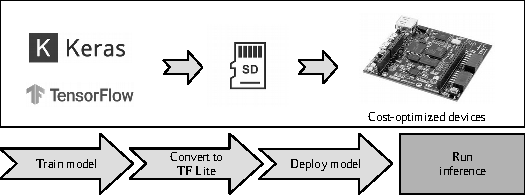
\includegraphics[width=0.5\textwidth]{../figures/workflow.pdf}
	\caption{The workflow of our approach on embedded FPGAs.}
	\label{fig:workflow}
\end{figure}

Our main contributions are as follows:
\begin{enumerate}
	\item We present the Hybrid-Float6 quantization. This approach improves generalization by reducing over-fit on feature extraction. The HF6 is wrapped into the standard floating-point representation (IEEE 754) allowing compatibility with standard hardware. Therefore, it can be beneficial for inference in other devices.
	\item We develop a hardware/software co-design framework for sensor analytics applications on low-power and resource-limited FPGAs. This is a scalable architecture integrating TensorFlow Lite core in the embedded system.
	\item We present a customizable tensor processor as a dedicated hardware for HF6. This design computes \emph{Conv2D} tensor operations employing a pipelined vector dot-product with parametrized on-chip memory utilization. The compute engine of the tensor processor is implemented with standard floating-point, fixed-point, and HF6.
	\item We demonstrate the potential of our approach by addressing CNN model and hardware design exploration for sensor analytics of anomaly localization based on regression for SHM. We evaluate inference accuracy, compute performance, hardware resource utilization, and energy consumption.
\end{enumerate}

The rest of the paper is organized as follows. Section~\ref{sec:related_work} covers the related work; Section~\ref{sec:background} introduces the background to \emph{Conv2D} and \emph{DepthwiseConv2D} tensor operations; Section~\ref{sec:system_design} describes the system design of the hardware/software architecture and the quantized aware training method; Section~\ref{sec:experimental_results} presents the experimental results thorough a design exploration flow; Section~\ref{sec:conclusions} concludes the paper.

This design exploration framework is available to the community as an open-source project at (\emph{hidden for double blinded review}).